\bigskip

\item The functions plotted below are all of the form $y = A \sin(B x + C)$. Which function has the largest value of $B$?

% \resizebox{6in}{!}{\includegraphics{SVC.01.05.070.ps}}
    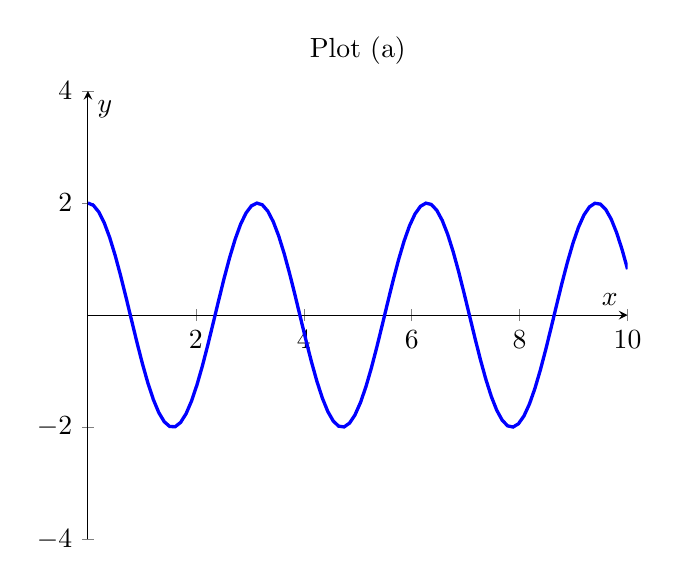
\begin{tikzpicture}
        \begin{axis}[axis lines=center, xlabel={$x$}, ylabel={$y$}, xmin=0, xmax=10,
                ymin=-4, ymax=4, domain=0:10, samples=100, title={Plot (a)}]
                \addplot[color=blue, very thick] {2*cos(2*deg(x))};
            \end{axis}
        \end{tikzpicture}
    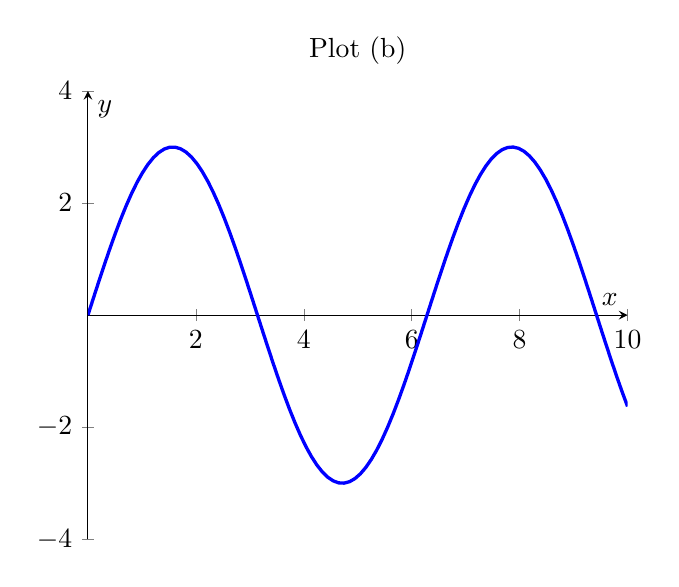
\begin{tikzpicture}
        \begin{axis}[axis lines=center, xlabel={$x$}, ylabel={$y$}, xmin=0, xmax=10,
                ymin=-4, ymax=4, domain=0:10, samples=100, title={Plot (b)}]
                \addplot[color=blue, very thick] {3*sin(deg(x))};
            \end{axis}
        \end{tikzpicture}\\
    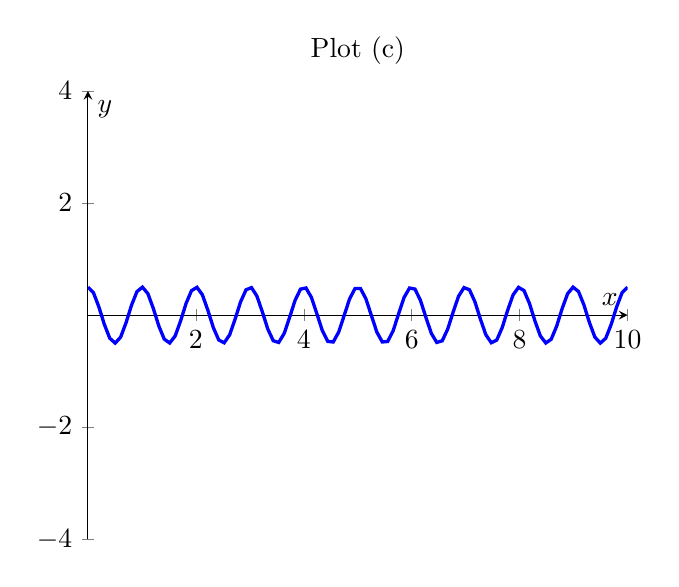
\begin{tikzpicture}
        \begin{axis}[axis lines=center, xlabel={$x$}, ylabel={$y$}, xmin=0, xmax=10,
                ymin=-4, ymax=4, domain=0:10, samples=100, title={Plot (c)}]
                \addplot[color=blue, very thick] {0.5*cos(2*pi*deg(x))};
            \end{axis}
        \end{tikzpicture}
    \begin{tikzpicture}
        \begin{axis}[axis lines=center, xlabel={$x$}, ylabel={$y$}, xmin=0, xmax=10,
                ymin=-4, ymax=4, domain=0:10, samples=100, title={Plot (d)}]
                \addplot[color=blue, very thick] {2*sin(2*pi/20*deg(x))};
            \end{axis}
        \end{tikzpicture}

% Carroll College MathQuest
